\documentclass{article}

\usepackage{graphicx}
\usepackage{amsmath, amsthm, amssymb}
\usepackage{pgfplots}
\pgfplotsset{compat=1.18} % Ensures backward compatibility
\usepackage{mdframed}
\usepackage{float}
\usepackage{xcolor}
\usepackage{tcolorbox}
\usepackage{hyperref} % Load this last in your preamble
\hypersetup{
    colorlinks=true,
    urlcolor=blue!70!black
}

\theoremstyle{definition}
\newtheorem{definition}{Definition}
\newtheorem{example}{Example}
\newcommand{\doenetlink}[2]{%
    \begin{tcolorbox}[
        colback=gray!6,
        colframe=blue!60!black,
        boxrule=0pt,
        leftrule=3pt,
        arc=2pt,
        left=8pt, right=8pt, top=6pt, bottom=6pt,
        before skip=10pt, after skip=10pt
    ]
    \textbf{\href{#2}{#1}} \\
    {\small\ttfamily \url{#2}}
    \end{tcolorbox}%
}

\title{Systems of Equations}
\author{}
\date{}

\begin{document}

\maketitle

% As you read through these notes, write down any questions you have. Posing clear questions is part of the practice of mathematics. If you have a question, it is likely that someone else has the same question. You can email me the questions or ask them at the beginning of class.

\section{Introduction}

We begin with a definition. Read it slowly a few times and try to understand what all of the symbols mean. Then, look at Example \ref{ex:linear-eqn-3var} and Example \ref{ex:linear-eqn-pt-slope} and make sure you see why each one fits the definition. Finally, look at Example \ref{ex:linear-eqn-non} and make sure you understand why those equations do not fit the definition.

\begin{definition} \label{def:linear-eqn}
A \textbf{linear equation in} $n$ \textbf{variables} is an equation that can be written in the form
\[a_1x_1+\cdots+a_nx_n=b\]
where $a_1, \ldots a_n, b$ are real numbers and \(n\) is a positive integer. The numbers \(a_1, \ldots, a_n\) are called \textbf{coefficients}. A \textbf{solution} to a linear equation in \(n\) variables is a list \((s_1, \ldots, s_n)\) of real numbers that makes the equation a true statement when the values \(s_1, \ldots, s_n\) are substituted for \(x_1, \ldots, x_n\), respectively.
\end{definition}

% \begin{example}
% The equation
% \[2x+3y=22\]
% is a linear equation in two variables. Using the notation in Definition \ref{def:linear-eqn}, we have \(a_1=2\), \(a_2=3\), \(b=22\), \(x_1=x\), and \(x_2=y\). Since \((5, 4)\) makes the equation a true statement when \(5\) is substituted for \(x\) and \(4\) is substituted for \(y\) (observe: \(2(5)+3(4)=22\)), the list \((5, 4)\) is a solution to \(2x+3y=22\). There are infinitely many others.
% \end{example}

\begin{example}\label{ex:linear-eqn-3var}
The equation
\[3x+5y-6z=10\]
is a linear equation in three variables. Using the notation in Definition \ref{def:linear-eqn}, we have \(a_1=3\), \(a_2=5\), \(a_3=-6\), \(b=10\), \(x_1=x\), \(x_2=y\), and \(x_3=z\). Since substituting \(2\) for \(x\), \(2\) for \(y\), and \(1\) for \(z\) makes the equation a true statement (observe: \(3(2)+5(2)-6(1)=10\)), the list \((2, 2, 1)\) is a solution to the equation. There are infinitely many others.
\end{example}

% \begin{example}
% The slope-intercept form of a line, \(y=mx+b\), is a linear equation in two variables. Take, for example, \(y=3x+5\). By subtracting \(3x\) from both sides and stating the coefficient of \(y\) explicitly we get
% \[-3x+1y=5,\]
% which matches the form in Definition \ref{def:linear-eqn} by taking \(a_1=-3\), \(a_2=1\), \(b=5\), \(x_1=x\), and \(x_2=y\). The list \((-1, 2)\) is a solution since \(-3(-1)+1(2)=5\). The line itself is a graphical representation of the infinitely many solutions \((s_1, s_2)\).
% \end{example}

\begin{example}\label{ex:linear-eqn-pt-slope}
The point-slope form of a line, \(y=y_0+m(x-x_0)\) is a linear equation in two variables. Take, for example, \(y=3+2(x-6)\). Using algebra, we can rewrite the equation in the form of Definition \ref{def:linear-eqn}:
\begin{align*}
    y=3+2(x-6) &\Longrightarrow y=3+2x-12 \\
    &\Longrightarrow y=2x-9 \\
    &\Longrightarrow -2x+y=-9.
\end{align*}
Using the notation in Definition \ref{def:linear-eqn}, we have \(a_1=-2\), \(a_2=1\), \(b=-9\), \(x_1=x\), and \(x_2=y\). The line itself is a graphical representation of the infinitely many solutions \((s_1, s_2)\).
\end{example}

\begin{example}\label{ex:linear-eqn-non}
The equations \(x^2+x+1=0\), \(4x-xy=2\), \(5\sqrt{x}=2\), and \(3x+\frac{1}{y}=y\) are \textit{not} linear equations. The terms \(x^2\), \(xy\), \(\sqrt{x}\), and \(\frac{1}{y}\) prohibit them from being rewritten in the form in Definition \ref{def:linear-eqn}.
\end{example}

\subsection{Preview Activity}

Click the link or URL below to access the Preview Activity for this section. You must be logged in to Doenet for your score to be recorded. If you click the link and are taken to a page that says \textbf{Taking assignment as an anonymous user}, you are \textit{not} logged in. If that happens, click the circle with the question mark and select \textbf{Sign in to save work}. After completing the sign-in process, return here and click the link again.

\doenetlink{Systems of Equations 1 Preview Activity}{https://doenet.org/code/737878}


\section{Systems of Linear Equations}

\begin{definition}
A \textbf{system of linear equations} is a collection of one or more linear equations involving the same variables:
\begin{align*}
    a_{11}x_1+\cdots+a_{1n}x_n&=b_1 \\
    &\vdots \\
    a_{k1}x_1+\cdots+a_{kn}x_n&=b_k.
\end{align*}
A \textbf{solution} of the system is a list \((s_1, \ldots, s_n)\) of numbers that is a solution to each of the equations in the system.
\end{definition}

\begin{example}
    Consider the system of linear equations
    \begin{align}
    \begin{split}
        -x+y&=-1 \\
        \frac{1}{2}x+y&=2.
    \end{split}
    \label{eqn:linear-system-1}
    \end{align}
    Figure \ref{fig:linear-system-1} shows the graphs of the linear equations (\ref{eqn:linear-system-1}). Each line represents the set of solutions to the corresponding linear equation. The lines share a single point, \((2, 1)\), which is the only solution to the system.

\begin{figure}[H]
    \centering
    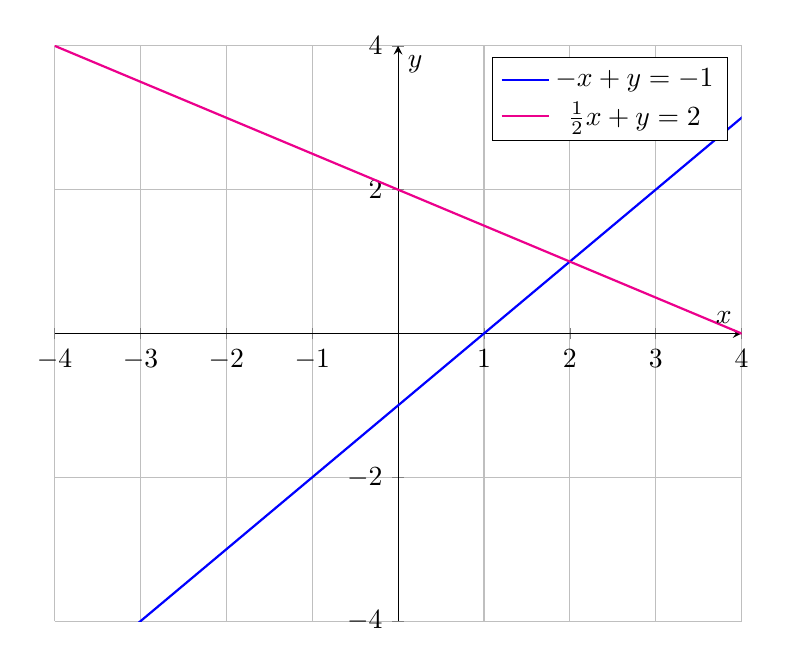
\begin{tikzpicture}
        \begin{axis}[
            axis lines = middle,    % Centers the axes like a standard math graph
            xlabel = {$x$},         % Label for the x-axis
            ylabel = {$y$},         % Label for the y-axis
            xmin=-4, xmax=4,        % Minimum and maximum x values displayed
            ymin=-4, ymax=4,       % Minimum and maximum y values displayed
            grid = major,           % Adds grid lines
            width=0.85\textwidth,
            % width=10cm,             % Width of the chart
            % height=10cm,             % Height of the chart
            % title={Graph of $y = 2x + 1$}
        ]
            % Plot the linear equation
            \addplot [
                domain=-5:5,        % The domain over which to calculate the line
                samples=2,          % Only 2 samples are needed for a perfect straight line
                color=blue,         % Line color
                thick,              % Line thickness
            ] {x - 1};            % The linear equation formula
            \addlegendentry{$-x+y=-1$}
            \addplot [
                domain=-5:5,        % The domain over which to calculate the line
                samples=2,          % Only 2 samples are needed for a perfect straight line
                color=magenta,         % Line color
                thick,              % Line thickness
            ] {-0.5*x + 2};              
            \addlegendentry{$\frac{1}{2}x+y=2$}
            
        \end{axis}
    \end{tikzpicture}
    \caption{The graphs of \(-x+y=-1\) and \(\frac{1}{2}x+y=2\) intersect at the point \((2, 1)\), the solution to the corresponding linear system.}
    \label{fig:linear-system-1}
\end{figure}
\end{example}

The system of equations in the previous example had a single solution, but this is not always the case. In fact, we have the following fact about systems of linear equations:

\begin{mdframed}[
    backgroundcolor=gray!15,
    linecolor=black,       % The dark border color
    linewidth=1pt,         % Border thickness
    innertopmargin=10pt,   % Margin inside the box at the top
    innerbottommargin=10pt,% Margin inside the box at the bottom
    userdefinedwidth=0.8\textwidth,
    align=center           % Centers the box on the page
]
A system of linear equations has either 1 solution, no solutions, or infinitely many solutions.
\end{mdframed}

\begin{example}
    Consider the system of linear equations
    \begin{align}
    \begin{split}
        x+z&=2 \\
        x+y-z&=0.
    \end{split}
    \label{eqn:linear-system-2}
    \end{align}    
    The solution set to each of the equations in (\ref{eqn:linear-system-2}) can be represented as a 2-dimensional plane in 3-dimensional space. The two planes intersect at a line, which represents the solution set of the system. See Figure \ref{fig:linear-system-2}.

\begin{figure}[H]
    \centering
    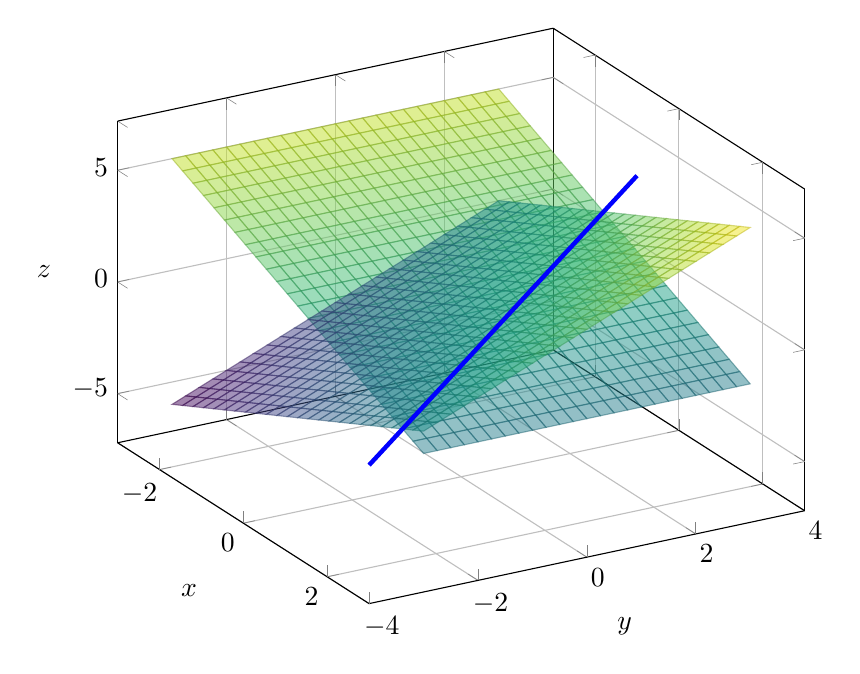
\begin{tikzpicture}
        \begin{axis}[
            width=0.85\textwidth,
            xlabel={$x$},
            ylabel={$y$},
            zlabel={$z$},
            zlabel style={rotate=-90, anchor=east},
            colormap/viridis, % A beautiful built-in color gradient
            view={60}{30},   % Changes the camera viewing angle (azimuth and elevation)
            grid=major
        ]
            % Plotting a mathematical function
            \addplot3[
                surf,         % Specifies a surface plot
                domain=-3:3,  % X range
                domain y=-3:3,% Y range
                opacity=0.5
            ] {2-x};

            \addplot3[
                surf,         % Specifies a surface plot
                domain=-3:3,  % X range
                domain y=-3:3,% Y range
                opacity=0.5
            ] {x+y};

            \addplot3[
                blue,          % Line color
                ultra thick,   % Make the line stand out
                samples y=0,   % Tells pgfplots this is a 1D line, not a 2D surface grid
                domain=-1:3,   % The range for your parameter 't'
                variable=t     % Defines 't' as the independent parameter
            ] (
                {t},           % x(t)
                {2 - 2*t},     % y(t) - use * for multiplication
                {2 - t}        % z(t)
            );
        \end{axis}
    \end{tikzpicture}
    \caption{Two planes and their line of intersection. Each plane represents the solutions to a linear equation in three variables; the line where they intersect represents the solutions to the corresponding system.}
    \label{fig:linear-system-2}
\end{figure}
\end{example}

\begin{example}
    Consider the system of linear equations
    \begin{align}
    \begin{split}
        -x+y&=-1 \\
        -x+y&=2.
    \end{split}
    \label{eqn:linear-system-2}
    \end{align}
    Figure \ref{fig:linear-system-2} shows the graphs of the linear equations (\ref{eqn:linear-system-2}). The system has no solution; equivalently, the lines do not intersect.

\begin{figure}[H]
    \centering
    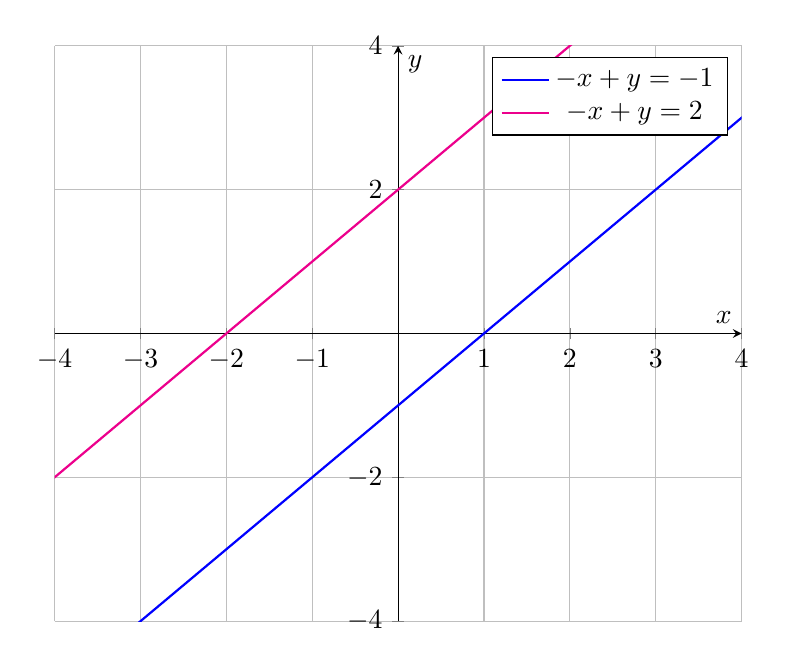
\begin{tikzpicture}
        \begin{axis}[
            axis lines = middle,    % Centers the axes like a standard math graph
            xlabel = {$x$},         % Label for the x-axis
            ylabel = {$y$},         % Label for the y-axis
            xmin=-4, xmax=4,        % Minimum and maximum x values displayed
            ymin=-4, ymax=4,       % Minimum and maximum y values displayed
            grid = major,           % Adds grid lines
            width=0.85\textwidth,
            % width=10cm,             % Width of the chart
            % height=10cm,             % Height of the chart
            % title={Graph of $y = 2x + 1$}
        ]
            % Plot the linear equation
            \addplot [
                domain=-5:5,        % The domain over which to calculate the line
                samples=2,          % Only 2 samples are needed for a perfect straight line
                color=blue,         % Line color
                thick,              % Line thickness
            ] {x - 1};            % The linear equation formula
            \addlegendentry{$-x+y=-1$}
            \addplot [
                domain=-5:5,        % The domain over which to calculate the line
                samples=2,          % Only 2 samples are needed for a perfect straight line
                color=magenta,         % Line color
                thick,              % Line thickness
            ] {x + 2};              
            \addlegendentry{$-x+y=2$}
            
        \end{axis}
    \end{tikzpicture}
    \caption{The graphs of \(-x+y=-1\) and \(-x+y=2\) do not intersect; the corresponding linear system has no solutions.}
    \label{fig:linear-system-2}
\end{figure}
\end{example}


\end{document}
